\documentclass[a4paper,11pt,oneside]{book}
% =====================================================================
% de_style.tex: Differential Equations (Ch11) homework / test layout.
% = Ch10 di_style (copied as de_core.tex; header text changed) + the DE
% notation and the framed solution boxes of the v1 DE documents
% (soln / spart, used by the Test worked solutions).
% =====================================================================
% =====================================================================
% di_style.tex: Differential Equations homework / test layout.
% Loads the house preamble (local copies of the AoI worksheet files:
% ws_preamble_build.tex, ws_preamble_local.tex -> ws_figstyles.tex),
% then adds the homework layout used by HW1-HW3 and the Test.
% Usage (before \begin{document}):  \ditle{Homework 1}
% =====================================================================
% WORKSHEET COPY of ../notes/preamble_build.tex (2026-10-09 version), unchanged.
% preamble_build.tex: copy of Maximus's preamble.tex for the DE v3 build.
% The blocks marked [BUILD COPY CHANGE] are the earlier build fixes.
% The blocks marked [V3 ADDITION] are new in this version (example box,
% spacing). Everything else is unchanged from preamble.tex.

% For margins
\usepackage[a4paper, margin = 20mm]{geometry}

\usepackage[Lenny]{fncychap}
% Rejne, Glenn, Lenny

\usepackage{etoc}

% [V3 ADDITION] cancel: used to show the dx's "cancelling" in Section 11.3
\usepackage{cancel}
\renewcommand{\CancelColor}{\color{red}}

% For enumeration & math symbols
\usepackage{enumerate}
\usepackage{amsmath,amsfonts,amssymb,amsthm,graphicx,lipsum}

% For diagrams, plots and boxes
\usepackage{pgfplots}
\pgfplotsset{compat=1.18}
\usepackage{tikz}
\usepackage[most]{tcolorbox}
\tcbuselibrary{skins}
\usepackage{xcolor}
\pgfplotsset{
    standard/.style={clip = false,
    axis line style = thick,
    trig format=rad,
    axis lines = middle,
    every axis x label/.style={at={(current axis.right of origin)},anchor= west},
    every axis y label/.style={at={(current axis.above origin)},anchor=south}
    }
}

% For GC font
\usepackage{fontspec}
% [BUILD COPY CHANGE 1] The TI-84 key font is loaded only if the file exists
% (checked in ./Fonts/... and ../Fonts/...). Otherwise \ti{} falls back to a
% small boxed sans-serif key. Known letters of the TI font are mapped to their
% key names in the fallback: o = [y=], z = [mode], f = [L3].
\newcommand{\tikey}[1]{\tcbox[on line, enhanced, boxsep=0pt, left=2pt, right=2pt,
  top=1pt, bottom=1pt, boxrule=0.5pt, arc=1.5pt, colback=white,
  colframe=black!70]{\sffamily\footnotesize\strut #1}}
\ExplSyntaxOn
\NewDocumentCommand{\tifallback}{m}{
  \str_case:nnF {#1}
    { {o}{\tikey{y=}} {z}{\tikey{mode}} {f}{\tikey{L3}} }
    { \tikey{#1} }
}
\ExplSyntaxOff
\def\tifontcase{0}
\IfFileExists{Fonts/TI-84 Plus CE Key Fonts/TI84PlusCEKeys.ttf}
  {\def\tifontcase{1}}{}
\IfFileExists{../Fonts/TI-84 Plus CE Key Fonts/TI84PlusCEKeys.ttf}
  {\def\tifontcase{2}}{}
\ifcase\tifontcase\relax
  % 0: font not found, use boxed fallback keys
  \newcommand{\ti}[1]{\tifallback{#1}}
\or
  % 1: original location (as in preamble.tex)
  \newfontfamily\tifont[
    Path = {Fonts/TI-84 Plus CE Key Fonts/},
    UprightFont = {TI84PlusCEKeys.ttf}
  ]{}
  \newcommand{\ti}[1]{{\tifont #1}}
\or
  % 2: one level up (when compiling inside draft-ch1/)
  \newfontfamily\tifont[
    Path = {../Fonts/TI-84 Plus CE Key Fonts/},
    UprightFont = {TI84PlusCEKeys.ttf}
  ]{}
  \newcommand{\ti}[1]{{\tifont #1}}
\fi

% [AoI items 17/18/37] GC DISPLAY FONT. Every GC key, command, menu item and
% screen line goes through \gcfont, so the font can be swapped HERE in one place.
%   \gc{fnInt(}      command / menu item / stored variable in the display font
%   \gckey{2nd}      a calculator key (display font in a small key outline)
%   \gcscreen{...}   a calculator screen (display font on a grey-green LCD panel)
% The font file lives in ../Fonts (shared by notes, slides and worksheet).
\def\gcfontfile{VT323-Regular.ttf}
\IfFileExists{../Fonts/\gcfontfile}{%
  \newfontfamily\gcfont[Path=../Fonts/, Scale=1.32]{\gcfontfile}}{%
  \newcommand\gcfont{\ttfamily}}
\newcommand{\gc}[1]{\mbox{\gcfont #1}}
\newcommand{\gckey}[1]{\tcbox[on line, enhanced, boxsep=0pt, left=2pt, right=2pt,
  top=0.6pt, bottom=0.2pt, boxrule=0.5pt, arc=1.5pt, colback=black!4,
  colframe=black!65]{\gcfont\strut #1}}
\definecolor{lcd}{RGB}{214,222,204}
\newcommand{\gcscreen}[1]{\tcbox[on line, enhanced, boxsep=1pt, left=4pt, right=4pt,
  top=2pt, bottom=2pt, boxrule=1.2pt, arc=1pt, colback=lcd, colframe=black!70]{%
  \gcfont\begin{tabular}{@{}l@{}}#1\end{tabular}}}
% integral template as shown on the TI-84 Plus CE (MathPrint): \gcint{0}{2}{e^(-X²)}{X}
\newcommand{\gcint}[4]{{\gcfont\raisebox{-0.35ex}{\Large ∫}\hspace{-0.15em}%
  \raisebox{-0.2ex}{\begin{tabular}{@{}l@{}}\footnotesize #2\\[-1.3ex]\footnotesize #1\end{tabular}}%
  \hspace{0.1em}(#3)\mathrm{d}#4}}
% old key macro kept as an alias so nothing breaks
\renewcommand{\ti}[1]{\gckey{#1}}

% SI units
\usepackage{siunitx}

% setspace
%\usepackage{setspace}
%\onehalfspacing

% For hyperlinks within and out of document
\usepackage{hyperref}
\hypersetup{
    colorlinks = true,
    linkcolor = black,
    urlcolor = blue,
}   

% For captions for pics
\usepackage{capt-of}


% tcolorbox custom environments
% Definition ========================================================
\newtcolorbox[auto counter,number within=section]{definition}[2][drop shadow]{%
enhanced, before skip=5mm, after skip=6mm, % [V3 ADDITION] spacing
colback=blue!5!white,colframe=blue!50!black,fonttitle=\bfseries,
title= Definition~\thetcbcounter. #2,#1}

% Theorem ==========================================================
\newtcolorbox[auto counter,number within=section]{theorem}[2][drop shadow]{%
enhanced, before skip=5mm, after skip=6mm, % [V3 ADDITION] spacing
colback=black!5!white,colframe=black,fonttitle=\bfseries,
title= Theorem~\thetcbcounter. #2,#1}

% Caution box ======================================================
\newtcolorbox{caution}[1][]{enhanced,
before skip=5mm,after skip=6mm, % [V3 ADDITION] was 2mm/3mm
boxrule=1pt,left=11mm,right=2mm,top=3mm,bottom=3mm,
colback=yellow!50,
colframe=yellow!20!black,
sharp corners,rounded corners=southeast,arc is angular,arc=3mm,
underlay={%
\path[fill=tcbcolback!80!black] ([yshift=3mm]interior.south east)--++(-0.4,-0.1)--++(0.1,-0.2);
\path[draw=tcbcolframe,shorten <=-0.05mm,shorten >=-0.05mm] ([yshift=3mm]interior.south east)--++(-0.4,-0.1)--++(0.1,-0.2);
\path[fill=yellow!50!black,draw=none] (interior.south west) rectangle node[white]{\Huge\bfseries !} ([xshift=9mm]interior.north west);
},
drop fuzzy shadow,#1}

% Question box ======================================================
\newtcolorbox{question}[1][]{enhanced,
before skip=5mm,after skip=6mm, % [V3 ADDITION] was 2mm/3mm
boxrule=1pt,left=11mm,right=2mm,top=3mm,bottom=3mm,
colback=blue!20!white,
colframe=blue!20!black,
sharp corners,rounded corners=southeast,arc is angular,arc=3mm,
underlay={%
\path[fill=tcbcolback!80!black] ([yshift=3mm]interior.south east)--++(-0.4,-0.1)--++(0.1,-0.2);
\path[draw=tcbcolframe,shorten <=-0.05mm,shorten >=-0.05mm] ([yshift=3mm]interior.south east)--++(-0.4,-0.1)--++(0.1,-0.2);
\path[fill=blue!50!black,draw=none] (interior.south west) rectangle node[white]{\Huge\bfseries ?} ([xshift=9mm]interior.north west);
},
drop fuzzy shadow,#1}

% Information box ======================================================
\newtcolorbox{info}[1][]{enhanced,
before skip=5mm,after skip=6mm, % [V3 ADDITION] was 2mm/3mm
boxrule=1pt,left=11mm,right=2mm,top=3mm,bottom=3mm,
colback=cyan!20!white,
colframe=cyan!20!black,
sharp corners,rounded corners=southeast,arc is angular,arc=3mm,
underlay={%
\path[fill=tcbcolback!80!black] ([yshift=3mm]interior.south east)--++(-0.4,-0.1)--++(0.1,-0.2);
\path[draw=tcbcolframe,shorten <=-0.05mm,shorten >=-0.05mm] ([yshift=3mm]interior.south east)--++(-0.4,-0.1)--++(0.1,-0.2);
\path[fill=cyan!50!black,draw=none] (interior.south west) rectangle node[white]{\Huge\bfseries i} ([xshift=9mm]interior.north west);
},
drop fuzzy shadow,#1}

% Mistake box ======================================================
\newtcolorbox{mistake}[1][]{enhanced,
before skip=5mm,after skip=6mm, % [V3 ADDITION] was 2mm/3mm
boxrule=1pt,left=11mm,right=2mm,top=3mm,bottom=3mm,
colback=red!20!white,
colframe=red!20!black,
sharp corners,rounded corners=southeast,arc is angular,arc=3mm,
underlay={%
\path[fill=tcbcolback!80!black] ([yshift=3mm]interior.south east)--++(-0.4,-0.1)--++(0.1,-0.2);
\path[draw=tcbcolframe,shorten <=-0.05mm,shorten >=-0.05mm] ([yshift=3mm]interior.south east)--++(-0.4,-0.1)--++(0.1,-0.2);
\path[fill=red!50!black,draw=none] (interior.south west) rectangle node[white]{\Huge\bfseries $\times$} ([xshift=9mm]interior.north west);
},
drop fuzzy shadow,#1}



% [V3 ADDITION] Worked example box ==================================
% Own counter, numbered within the section (Example 11.2.1, 11.2.2, ...).
% For per-subsection numbering (11.2.1.1) change `section' to `subsection'. Blue `question' boxes are kept for thought-provoking questions
% only; worked examples always use this box. Usage:
%   \begin{example} ...question text... \end{example}
%   \solution{...}
\newtcolorbox[auto counter,number within=section]{example}[1][]{%
enhanced, breakable=false, before skip=5mm, after skip=4mm,
colback=teal!5!white, colframe=teal!55!black, boxrule=0.8pt,
left=3mm, right=3mm, top=2mm, bottom=2mm,
sharp corners, rounded corners=northwest, arc=3mm,
fonttitle=\bfseries, coltitle=white,
title=Example~\thetcbcounter, attach boxed title to top left={yshift=-2mm, xshift=3mm},
boxed title style={colback=teal!55!black, sharp corners, rounded corners=northwest, arc=2mm},
drop fuzzy shadow, #1}

% [V3 ADDITION] Spacing between sections, subsections, parts, paragraphs =
% (fncychap's chapter heading is untouched; only \section and below.)
\makeatletter
\renewcommand\section{\@startsection{section}{1}{\z@}%
  {-2ex \@plus -.5ex \@minus -.2ex}{3.2ex \@plus .3ex}%
  {\normalfont\LARGE\bfseries\color{blue!50!black}}}
\renewcommand\subsection{\@startsection{subsection}{2}{\z@}%
  {-1.5ex \@plus -.5ex \@minus -.2ex}{2.6ex \@plus .3ex}%
  {\normalfont\Large\bfseries}}
\renewcommand\subsubsection{\@startsection{subsubsection}{3}{\z@}%
  {-4ex \@plus -1ex \@minus -.5ex}{1.6ex \@plus .2ex}%
  {\normalfont\large\bfseries\color{teal!50!black}}}
\makeatother
\setlength{\parindent}{0pt}
\setlength{\parskip}{0.9ex plus 0.3ex minus 0.2ex}

% Headers and Footers
\usepackage{fancyhdr,lastpage}
% [V3 R2] grey left-margin line on the out-of-syllabus pages (item 13)
\usepackage{eso-pic}
% [AoI item 63] thicker line (2.6pt, was 1.6pt) that starts just BELOW the header rule
% (top 14mm of the page left clear). Flag: copy this line into every chapter's preamble.
\newcommand{\oosmargin}{\AddToShipoutPictureBG{\put(12mm,0){\color{gray!75}\rule{2.6pt}{\dimexpr\paperheight-14mm\relax}}}}
\pagestyle{fancy}
\lhead{Maximus Pung Jun}
% [BUILD COPY CHANGE 2] Header bug fix: \chaptername is the word "Chapter",
% so the original header printed "Chapter 1: Chapter". \chaptermark now stores
% the bare chapter title in \leftmark, and the header uses \leftmark.
\renewcommand{\chaptermark}[1]{\markboth{#1}{}}
\rhead{Chapter \thechapter: \leftmark}
% \cfoot{Page \thepage\  of \pageref{LastPage}} % buggy, does not appear on chapter pages.

% [V3 R2] tick and cross markers for mistake boxes (G3)
\newcommand{\wrong}{\textcolor{red!70!black}{\ensuremath{\boldsymbol{\times}}}}
\newcommand{\cmark}{\textcolor{green!50!black}{\ensuremath{\checkmark}}}

\newcommand{\xmark}{\wrong}   % alias: red cross
% [V3 R2] out-of-syllabus helpers (DE notes item 13)
%   \oosmargin    : grey line in the left margin on every following page
%   \oosmarginoff : stop the margin line
%   \oosnote      : grey banner "Out of syllabus. For your interest only."
%   outofsyllabus : environment = new page + margin line + banner; ends with
%                   \clearpage and switches the margin line off again
\newcommand{\oosmarginoff}{\ClearShipoutPictureBG}
\newcommand{\oosnote}[1][Nothing in this section is examined in H2 Mathematics.]{\par\noindent\colorbox{gray!15}{\parbox{\dimexpr\textwidth-2\fboxsep}{\textbf{Out of syllabus. For your interest only.} #1}}\par}
\newenvironment{outofsyllabus}{\clearpage\oosmargin}{\clearpage\oosmarginoff}

% Notation as in Maximus's notes: italic d, display style everywhere (G1).
% Fractions inside exponents stay small, so never use these macros inside ^{}.
\newcommand{\dydx}{\dfrac{\mathrm{d}y}{\mathrm{d}x}}
\newcommand{\dvdx}{\dfrac{\mathrm{d}v}{\mathrm{d}x}}
\newcommand{\dudx}{\dfrac{\mathrm{d}u}{\mathrm{d}x}}
\newcommand{\ddydx}{\dfrac{\mathrm{d}^{2}y}{\mathrm{d}x^{2}}}
\newcommand{\ddt}[1]{\dfrac{\mathrm{d}#1}{\mathrm{d}t}}
% Small syllabus flag (no longer used in the DE notes, kept for other chapters)
\newcommand{\syllabusflag}[1]{\par\noindent{\footnotesize\color{red!70!black}\textbf{Syllabus note.} #1}\par}


% Teacher's copy toggle ================================================
% [BUILD COPY CHANGE 3] \ifx compares the whole word (the original
% \if\conform test was always false). DE_notes_student.tex predefines
% \conform as HideSolutions.
% A student copy defines \conform as HideSolutions BEFORE loading this preamble.
\providecommand\conform{ShowSolutions}
\newcommand\ShowSolutionsKey{ShowSolutions}
% [V3 ADDITION] In the student copy the hidden solution leaves stretchable
% blank space (\vfill), so the free space on each page is shared out as
% working space below the examples instead of collecting at the bottom.
% [AoI item 10] "Solution." on its own line, so that (a), (b), (c) line up below it.
\newcommand\solution[1]{\ifx\conform\ShowSolutionsKey
  \par\noindent\textbf{Solution.}\par\nobreak\vspace{0.5ex}\noindent #1\par\medskip\else\par\vspace{\workspace}\fi}
% [V3 R2] minimum working space left under each example in the student copy
\newlength\workspace\setlength\workspace{3cm plus 1fill}


\newcommand{\NN}{\mathbb{N}}
\newcommand{\ZZ}{\mathbb{Z}}
\newcommand{\QQ}{\mathbb{Q}}
\newcommand{\RR}{\mathbb{R}}
\newcommand{\CC}{\mathbb{C}}


% WORKSHEET COPY of ../notes/preamble_local.tex (version the worksheet was last built with,
% from ../_backup_pre_limitsum, 2026-10-09 17:31). Local so the worksheet no longer depends
% on ../notes; changes: \input{ws_figstyles}; [2026-10-09 follow-up] \mk marks now bold, as in the notes.
% =====================================================================
% preamble_local.tex: extra packages, styles and macros for the
% Applications of Integration chapter ONLY. Loaded after preamble_build.tex.
% Plot styles and the mini 3D macros are in figstyles.tex (shared with the
% slides and worksheets).
% =====================================================================
\usepgfplotslibrary{fillbetween}
\usepackage{adjustbox} % mini 3D pictures (figstyles.tex)
\usetikzlibrary{arrows.meta, decorations.pathreplacing, calc}
\input{ws_figstyles}

% Small fractions are allowed only in exponents and in the limits of an
% integral (which are superscripts/subscripts); everywhere else use \dfrac.
\newcommand{\dx}{\,\mathrm{d}x}
\newcommand{\dy}{\,\mathrm{d}y}
\newcommand{\evalat}[3]{\left[\,#1\,\right]_{#2}^{#3}}

% [item 78] right-aligned A-level style marks at the end of a question part
\newcommand{\mk}[1]{{\unskip\nobreak\hfil\penalty50\hskip1.5em\hbox{}\nobreak\hfill\textbf{[#1]}%
  \parfillskip=0pt\finalhyphendemerits=0\par}}
% [item 11] visually emphasised step labels in worked solutions
\newcommand{\step}[1]{\textcolor{teal!55!black}{\textbf{Step #1}}\quad}
% (a), (b), (c) part lists inside questions and solutions
\newenvironment{parts}{\begin{enumerate}[(a)]\setlength{\itemsep}{0.4ex}}{\end{enumerate}}
% SEAB-style solution layout (approved 10.5.8 template): working on the
% left, region sketch on the right (mini 3D pictures go under the sketch)
\newcommand{\solpair}[3][0.56]{\noindent\begin{minipage}[t]{#1\textwidth}\vspace{0pt}#2\end{minipage}\hfill
  \begin{minipage}[t]{\dimexpr0.98\textwidth-#1\textwidth\relax}\vspace{0pt}\centering #3\end{minipage}\par}
% minus-diagram style (drafts/minus_style_template.tex, items 29/31/62)
\pgfplotsset{minus/.style={axis lines=middle, width=5.0cm, height=4.2cm, ticks=none,
  xlabel={$x$}, ylabel={$y$}, every axis x label/.style={at={(ticklabel* cs:1)},anchor=west},
  every axis y label/.style={at={(ticklabel* cs:1)},anchor=south}, clip=false, axis on top,
  axis line style={gray!70}, every axis label/.append style={gray},
  every node/.append style={text=gray!80!black, font=\footnotesize}}}
\tikzset{hlreg/.style={fill=hl!35, draw=hl, thick}}

% =====================================================================
% prelim_fonts.tex: fonts of the real 9758 prelim papers (Word + MathType; pdffonts on
% ACJC 2026 P1/P2, ACJC 2025 P1, JPJC 2026, RVHS 2026, CJC/DHS/TJC/NYJC/HCI/EJC 2025):
%   text Times New Roman; cover/footer Arial; RI page footer Calibri (here Carlito);
%   maths = MathType: Times New Roman letters/digits (italic variables; upright digits,
%   function names, d, e, f), SymbolMT for the integral, sigma, pi and = + < >,
%   scripts 7 pt on 12 pt (about 58 %), tight operator spacing.
% Candidate C (teacher-approved 13 Oct 2026): the real Times New Roman and Arial
% (ttf-mscorefonts-installer) + URW Standard Symbols PS (fonts-urw-base35, a SymbolMT
% clone with the same Symbol encoding) for the integral, sigma, pi, = + < >;
% TeX Gyre Termes Math only for what MathType draws itself (radicals, stretchy brackets,
% fraction bars, arrows). House style: upright d (\mathrm{d}x), upright e and f.
% Loaded once by di_style / de_core (HW sheets) and prelim_style (Tests, solutions).
% =====================================================================
\ifdefined\prelimfontsloaded\endinput\fi
\def\prelimfontsloaded{1}
\edef\pfrestoreat{\catcode`\noexpand\@=\the\catcode`\@\relax}\makeatletter
% MathType script sizes: 7 pt superscripts on 12 pt text (58 %), 5 pt second level
\DeclareMathSizes{12}{12}{7}{5}
\DeclareMathSizes{11}{11}{6.5}{5}
\DeclareMathSizes{10.95}{10.95}{6.5}{5}
\DeclareMathSizes{10}{10}{6}{5}
\DeclareMathSizes{9}{9}{5.5}{5}
\DeclareMathSizes{14.4}{14.4}{8.5}{6}
\setmainfont{Times New Roman}
\setsansfont{Arial}
\newfontfamily\coverfont{Arial}
\newfontfamily\calibrifont{Carlito}
\usepackage{unicode-math}
\setmathfont{TeX Gyre Termes Math}
\setmathfont[range={up/{latin,Latin,num}}]{Times New Roman}
\setmathfont[range={it/{latin,Latin}}]{Times New Roman Italic}
\setmathfont[range={bfup/{latin,Latin,num}}]{Times New Roman Bold}
\setmathfont[range={"002B,"003D,"003C,"003E}]{Standard Symbols PS}
\newfontfamily\pf@sym{Standard Symbols PS}
\newfontfamily\pf@symi[FakeSlant=0.21]{Standard Symbols PS}
% MathType-like spacing (tighter than TeX around = + -)
\AtBeginDocument{\thickmuskip=2.5mu plus 1mu\medmuskip=1.5mu plus 1mu\thinmuskip=3mu
% Symbol integral and sigma (18 pt at 12 pt text, as MathType), slanted Symbol pi
 \renewcommand{\int}{\mathop{\vcenter{\hbox{\pf@sym\fontsize{\fpeval{1.5*\f@size}}{0pt}\selectfont\char"F2}}}\nolimits}%
 \renewcommand{\sum}{\mathop{\vcenter{\hbox{\pf@sym\fontsize{\fpeval{1.5*\f@size}}{0pt}\selectfont\char"E5}}}\limits}%
 \renewcommand{\pi}{\mathord{\text{\pf@symi\char"70}}}}
\pfrestoreat
% Times New Roman + MathType-style maths (as the prelim papers)
\usepackage{needspace}
\usepackage{zref-savepos,zref-abspage}\makeatletter\zref@addprop{savepos}{abspage}\makeatother
\usepackage{array}

% ---- shortlist toggle ------------------------------------------------
% \ifshortlist true  -> only the questions in SHORTLIST.md (+ challenges)
% A wrapper file sets it with \def\setshortlist{1} before \input-ing the
% main file; the main file can also be edited to say \shortlisttrue.
\newif\ifshortlist
% Task 5: the FINAL homework (= former shortlist) is the default build. HWn.tex -> HWn.pdf.
% A wrapper that sets \def\setfull{1} builds the archive with all original questions.
\ifdefined\setfull\else\shortlisttrue\fi

\makeatletter
% ---- REVIEW build: highlight amended content ---------------------------
% A wrapper sets \def\setreview{1}. In review mode amended text is shaded
% yellow and carries a hover note (PDF tooltip / sticky note); otherwise the
% macros print the content plainly.
%   \chg{note}{inline content}        short inline change (no line breaks), text mode
%   \chgm{note}{math}                 the same inside math mode
%   \begin{chgblock}{note} ... \end{chgblock}   paragraph/display-level change
\newif\ifreview
\ifdefined\setreview \reviewtrue \fi
% hover notes are raw PDF annotations (xdvipdfmx \special; no extra packages).
% Keep notes plain ASCII; balanced parentheses are fine.
\newsavebox{\chg@box}
\newcommand{\chg@ann}[4]{% width, height, depth, note -> invisible markup annotation with a hover note
  \special{pdf:ann width #1 height #2 depth #3 << /Type /Annot /Subtype /Square /Border [0 0 0] /BS << /W 0 >> /C [1 0.85 0] /CA 0.01
    /T (Review) /Subj (Amendment) /Contents (#4) >>}}
\newcommand{\chg@sticky}[1]{\special{pdf:ann width 12pt height 12pt depth 0pt << /Type /Annot /Subtype /Text /Name /Comment
    /C [1 0.85 0] /T (Review) /Subj (Amendment) /Contents (#1) >>}}
\newcommand{\chg}[2]{\ifreview\sbox\chg@box{\colorbox{yellow!60}{#2}}%
  \leavevmode\rlap{\chg@ann{\the\wd\chg@box}{\the\ht\chg@box}{\the\dp\chg@box}{#1}}\usebox\chg@box\else#2\fi}
% \chgm{note}{math}: the same, for use INSIDE math mode (display style kept)
\newcommand{\chgm}[2]{\ifreview\mathchoice{\chg{#1}{$\displaystyle#2$}}{\chg{#1}{$\textstyle#2$}}{\chg{#1}{$\scriptstyle#2$}}{\chg{#1}{$\scriptscriptstyle#2$}}\else#2\fi}
\newtcolorbox{chgbox}[1]{enhanced, breakable, colback=yellow!35, colframe=yellow!35, boxrule=0pt, sharp corners,
  left=2pt, right=14pt, top=1pt, bottom=1pt, before skip=2pt, after skip=2pt,
  overlay first and middle={}, overlay last={}, overlay unbroken and first={\node[anchor=north east, inner sep=1pt] at (frame.north east) {\chg@sticky{#1}\hbox to 12pt{\vrule width 0pt height 12pt}};}}
% \chgnote{note}: just the sticky-note icon (e.g. inside a figure); nothing outside review mode
\newcommand{\chgnote}[1]{\ifreview\chg@sticky{#1}\hbox to 12pt{\vrule width 0pt height 12pt}\fi}
\newenvironment{chgblock}[1]{\ifreview\begin{chgbox}{#1}\fi}{\ifreview\end{chgbox}\fi}

% ---- header ---------------------------------------------------------
\newcommand\di@title{}
\makeatletter
\newcommand{\ditle}[1]{\gdef\di@title{#1}}
\fancypagestyle{di}{\fancyhf{}%
  \lhead{\small \di@title}%
  \rhead{\small Compiled by Maximus Pung Jun}%
  \cfoot{\small\thepage}%
  \renewcommand{\headrulewidth}{0.4pt}}
\pagestyle{di}
% title block on page 1, as in his Typst sheets
\newcommand{\dititleblock}[1][]{\thispagestyle{di}%
  {\LARGE\scshape \di@title}\par\smallskip
  {Compiled by Maximus Pung Jun}\par\ifx&#1&\else\smallskip{\small\textcolor{black!60}{#1}}\par\fi\medskip}
\makeatother
\newcommand{\disection}[1]{\par\bigskip\noindent{\Large\scshape #1}\par\medskip}

% ---- questions --------------------------------------------------------
% \Qhead{label}{source tag}: question heading, tag in brackets on the right
\newcommand{\Qhead}[2]{\par\needspace{8\baselineskip}\bigskip\noindent
  {\large\bfseries #1}\hfill{\small\textcolor{black!60}{[#2]}}\par\smallskip}
% part lists with bold labels as he writes them: \pt{(a)}, \pt{(i)}, \pt{(b) (i)}
\newenvironment{qparts}[1][2.4em]{\begin{list}{}{\setlength\leftmargin{#1}%
  \setlength\labelwidth{\dimexpr#1-0.5em\relax}\setlength\labelsep{0.5em}%
  \setlength\itemsep{0.8ex}\setlength\topsep{0.6ex}\setlength\parsep{0.6ex}%
  \renewcommand\makelabel[1]{\textbf{##1}\hfil}}}{\end{list}}
\newcommand{\pt}[1]{\item[#1]}
% thin horizontal label for a challenge question
\newcommand{\challengebanner}{\par\bigskip\noindent\textcolor{black!50}{\rule[0.5ex]{\linewidth}{0.4pt}}\par
  \noindent{\large\scshape Challenge (optional)}\par}
% upright "units"
\newcommand{\units}[1]{\ \text{units}^{#1}}
% END line
\newcommand{\diend}[1][END OF WORKSHEET]{\par\vspace{2\baselineskip}\begin{center}\textbf{#1}\end{center}}

% ---- question registry (full / shortlist from one source) -------------
% \defQ{n}{tag}{body}   question n of the original sheet
% \defA{n}{answer body} its final answer, as printed in his answer section
% \putQ{n} / \putC{n}   print question n as the next (challenge) question
% \putA{n}              print its answer under the same new label
\newcounter{diq}
\makeatletter
\newcommand{\defQ}[3]{\expandafter\gdef\csname diQtag@#1\endcsname{#2}%
  \expandafter\long\expandafter\gdef\csname diQbody@#1\endcsname{#3}}
\newcommand{\defA}[2]{\expandafter\long\expandafter\gdef\csname diA@#1\endcsname{#2}}
\newcommand{\di@tag}[1]{\csname diQtag@#1\endcsname}% source tag only (no original Q number)
% A question never breaks across pages: it is measured and starts on a new page unless it
% fits whole on the rest of this one (only a question taller than a page may break, and then
% only between parts). Page positions of its start/end (zref labels q-s<n>/q-e<n> in the .aux)
% let the checker verify this.
\newsavebox{\di@qmeas}
\newcommand{\di@placeQ}[1]{\par\setbox\di@qmeas=\vbox{#1}%
  \ifdim\dimexpr\ht\di@qmeas+\dp\di@qmeas\relax<0.95\textheight
    \needspace{\dimexpr\ht\di@qmeas+\dp\di@qmeas+\bigskipamount\relax}\else\needspace{14\baselineskip}\fi
  \zsavepos{q-s\thediq}#1\par\zsavepos{q-e\thediq}}
\newcommand{\putQ}[1]{\stepcounter{diq}%
  \expandafter\xdef\csname diLab@#1\endcsname{\thediq}%
  \di@placeQ{\Qhead{\thediq}{\di@tag{#1}}\csname diQbody@#1\endcsname\par}}
\newcommand{\putC}[1]{\stepcounter{diq}%
  \expandafter\xdef\csname diLab@#1\endcsname{\thediq}%
  \expandafter\gdef\csname diChal@#1\endcsname{1}%
  \di@placeQ{\Qhead{\thediq\quad\normalsize\mdseries\scshape Challenge}{\di@tag{#1}}\csname diQbody@#1\endcsname\par}}
\newcommand{\putA}[1]{\par\needspace{4\baselineskip}%
  \begin{qparts}[2.4em]\item[{\csname diLab@#1\endcsname}]\csname diA@#1\endcsname\end{qparts}\medskip}
% ---- worked solutions: \defS{n}{body}, \putQS{n} prints question n + its solution ----
\newcommand{\defS}[2]{\expandafter\long\expandafter\gdef\csname diS@#1\endcsname{#2}}
\newcommand{\disolhead}{\par\medskip\noindent{\bfseries Solution}\par\nobreak\vspace{-0.6ex}\noindent\textcolor{black!35}{\rule{\linewidth}{0.4pt}}\par\nobreak}
\newcommand{\putQS}[1]{\putQ{#1}\disolhead\csname diS@#1\endcsname\par}
% source of a worked solution; visible only in REVIEW builds. #1: his / pub / pip
\newcommand{\solsrc}[2]{\ifreview\par\noindent\def\di@a{#1}\def\di@b{pip}%
  \ifx\di@a\di@b\colorbox{yellow!60}{\parbox{\dimexpr\linewidth-2\fboxsep-14pt}{\small\textbf{Pip-worked:} #2}}\chgnote{Pip-worked solution. No worked solution by the teacher and no published solution was found. Please check it.}%
  \else{\small\textcolor{black!55}{Source of this solution: #2}}\fi\par\smallskip\fi}
\makeatother
% compact sketch for worked solutions: \solfig[axis options]{plot commands}
\newcommand{\solfig}[2][]{\par\begin{center}\begin{tikzpicture}\begin{axis}[qfig, width=6.6cm, height=5cm, #1]#2\end{axis}\end{tikzpicture}\end{center}}
% a sketch added to an existing worked solution (teacher rule), shaded in REVIEW
\newenvironment{addedsketch}{\begin{chgblock}{Sketch added: teacher rule - every area or volume solution has a sketch.}}{\end{chgblock}}
% answer part list (compact)
\newenvironment{aparts}[1][2.4em]{\begin{qparts}[#1]\setlength\itemsep{0.3ex}}{\end{qparts}}

% ---- figure helpers ---------------------------------------------------------
\tikzset{rect/.style={fill=blue!10, draw=blue!55!black, thin}}
\pgfplotsset{qfig/.style={sketch, every node/.append style={font=\scriptsize}}}
% aligned working that starts on the same line as a part label: \pt{(iii)} \begin{topalign} ... \end{topalign}
\newenvironment{topalign}{\hfill$\displaystyle\begin{aligned}[t]}{\end{aligned}$\hfill\null\par\smallskip}
% one display that starts on the same line as a part label
\newcommand{\topdisplay}[1]{\hfill$\displaystyle #1$\hfill\null\par\smallskip}

\providecommand{\prelimtitle}{DIFFERENTIAL EQUATIONS TEST}
\providecommand{\prelimsubject}{Differential Equations}
\providecommand{\e}{\mathrm{e}}
\providecommand{\cosec}{\operatorname{cosec}}
\providecommand{\dt}{\,\mathrm{d}t}
\providecommand{\abs}[1]{\left|#1\right|}
\providecommand{\dd}[2]{\dfrac{\mathrm{d}#1}{\mathrm{d}#2}}
\providecommand{\dvdx}{\dfrac{\mathrm{d}v}{\mathrm{d}x}}
\providecommand{\dudx}{\dfrac{\mathrm{d}u}{\mathrm{d}x}}
\colorlet{notegrey}{black!60}
\makeatletter
\protected\def\note#1{\ifmmode\text{\small\color{notegrey}\itshape #1}\else{\small\color{notegrey}\itshape #1}\fi}
\newcommand{\award}[1]{\unskip\nobreak\hfill\textbf{\small #1}}
\newcommand{\tagm}[1]{\tag*{\textbf{\small #1}}}
\newcommand{\mfAminus}{\[\begin{aligned}&\int\dfrac{1}{a^{2}-x^{2}}\dx\\&\quad=\dfrac{1}{2a}\ln\abs{\dfrac{a+x}{a-x}}+c\end{aligned}\]}
\newcommand{\mfXminus}{\[\begin{aligned}&\int\dfrac{1}{x^{2}-a^{2}}\dx\\&\quad=\dfrac{1}{2a}\ln\abs{\dfrac{x-a}{x+a}}+c\end{aligned}\]}
\newcommand{\sbs@start}{\if@inlabel\def\sbs@shift{\vspace{-\ht\strutbox}}\else
  \ifvmode\else\par\fi\addvspace{0.4ex}\def\sbs@shift{}\fi\noindent}
\newsavebox{\sbs@box}
\newenvironment{sbs}[1]{%
  \sbs@start\begin{minipage}[t]{#1\linewidth}\vspace{0pt}\sbs@shift\raggedright%
  \def\sbsnext{\end{minipage}\hfill\begin{minipage}[t]{\dimexpr0.97\linewidth-#1\linewidth\relax}\vspace{0pt}\sbs@shift\setlength{\fboxsep}{1.5mm}\begin{lrbox}{\sbs@box}\begin{minipage}[t]{\dimexpr\linewidth-2\fboxsep-1pt\relax}\small\raggedright}%
}{\end{minipage}\end{lrbox}\setlength{\fboxrule}{0.5pt}\fbox{\usebox{\sbs@box}}\end{minipage}\par}
\newenvironment{sbsplain}[1]{%
  \sbs@start\begin{minipage}[t]{#1\linewidth}\vspace{0pt}\sbs@shift\raggedright%
  \def\sbsnext{\end{minipage}\hfill\begin{minipage}[t]{\dimexpr0.97\linewidth-#1\linewidth\relax}\vspace{0pt}\sbs@shift\centering}%
}{\end{minipage}\par}
% ---- framed worked-solution box (v1 DE mark-scheme layout, kept for the Test) ----
\newlength{\solcol}\setlength{\solcol}{15mm}
\newcounter{spartno}
\newcommand{\solskips}{\abovedisplayskip=4pt plus 2pt\belowdisplayskip=4pt plus 2pt\abovedisplayshortskip=2pt\belowdisplayshortskip=3pt}
\newtcolorbox{soln}[1][]{enhanced, breakable, sharp corners,
  colback=white, colframe=black, boxrule=0.6pt,
  boxsep=0pt, left=0pt, right=3mm, top=1.5mm, bottom=2mm,
  before skip=1.2ex, after skip=1.5ex,
  before upper={\setcounter{spartno}{0}\parskip=0.5ex\solskips\@fleqntrue\@mathmargin=0pt\raggedright},
  overlay={\draw[line width=0.4pt] ([xshift=\solcol]frame.north west) -- ([xshift=\solcol]frame.south west);},
  #1}
\newenvironment{spart}[1]{%
  \stepcounter{spartno}%
  \ifnum\value{spartno}>1 \par\vspace{0.2ex}\noindent
    \makebox[\linewidth][l]{\rule{\dimexpr\linewidth+3mm\relax}{0.4pt}}\par\nobreak\vspace{0.3ex}\fi
  \begin{list}{}{\leftmargin=\dimexpr\solcol+2.5mm\relax
    \labelwidth=\solcol \labelsep=2.5mm \itemindent=0pt
    \topsep=0.3ex \parsep=0.5ex \rightmargin=0pt \@beginparpenalty=\@M}%
  \item[{\makebox[\solcol][l]{\strut\hspace{1.5mm}\textbf{#1}}}]%
  \ignorespaces}{\end{list}}
\makeatother
% ---- DE sketches: thin light axes (teacher rule), as the Ch10 'sketch' style ----
\pgfplotsset{dsketch/.style={sketch, axis lines=middle, axis line style={thin, black!45, -{Stealth[length=1.6mm]}},
    ticks=none, clip=false, width=6.5cm, height=4.6cm,
    every axis x label/.style={at={(current axis.right of origin)},anchor=west},
    every axis y label/.style={at={(current axis.above origin)},anchor=south},
    every node/.append style={font=\small}},
  dcurve/.style={black, semithick, smooth, samples=120}}
\tikzset{asym/.style={black, dashed, thin}}
\makeatletter
\newcommand{\dstart}{\leavevmode\vadjust{\nobreak\vskip\dimexpr-\baselineskip-\abovedisplayskip+1pt\relax}}
\newcommand{\sdstart}{\leavevmode\vadjust{\nobreak\vskip\dimexpr-\baselineskip-\abovedisplayskip+4pt\relax}}
\makeatother

\usepackage{enumitem}\usepackage{multirow}\usepackage{makecell}\usepackage{array}
\defaultfontfeatures{Mapping=tex-text}
\def\prelimkeepcolour{1}
% =====================================================================
% prelim_style.tex: makes the Test look like a Singapore JC H2 Mathematics
% 9758 prelim paper (studied from ACJC/RI 2026 P1/P2 on the box:
% body Times New Roman + Times-style maths, cover in Arial).
% Fonts: prelim_fonts.tex (real Times New Roman/Arial + Times-style maths).
% Shared by Ch10 (di_style) and Ch11 (de_style; sets \prelimtitle/\prelimsubject). Loaded AFTER the chapter style (overrides its layout for the test only).
% =====================================================================
% =====================================================================
% prelim_fonts.tex: fonts of the real 9758 prelim papers (Word + MathType; pdffonts on
% ACJC 2026 P1/P2, ACJC 2025 P1, JPJC 2026, RVHS 2026, CJC/DHS/TJC/NYJC/HCI/EJC 2025):
%   text Times New Roman; cover/footer Arial; RI page footer Calibri (here Carlito);
%   maths = MathType: Times New Roman letters/digits (italic variables; upright digits,
%   function names, d, e, f), SymbolMT for the integral, sigma, pi and = + < >,
%   scripts 7 pt on 12 pt (about 58 %), tight operator spacing.
% Candidate C (teacher-approved 13 Oct 2026): the real Times New Roman and Arial
% (ttf-mscorefonts-installer) + URW Standard Symbols PS (fonts-urw-base35, a SymbolMT
% clone with the same Symbol encoding) for the integral, sigma, pi, = + < >;
% TeX Gyre Termes Math only for what MathType draws itself (radicals, stretchy brackets,
% fraction bars, arrows). House style: upright d (\mathrm{d}x), upright e and f.
% Loaded once by di_style / de_core (HW sheets) and prelim_style (Tests, solutions).
% =====================================================================
\ifdefined\prelimfontsloaded\endinput\fi
\def\prelimfontsloaded{1}
\edef\pfrestoreat{\catcode`\noexpand\@=\the\catcode`\@\relax}\makeatletter
% MathType script sizes: 7 pt superscripts on 12 pt text (58 %), 5 pt second level
\DeclareMathSizes{12}{12}{7}{5}
\DeclareMathSizes{11}{11}{6.5}{5}
\DeclareMathSizes{10.95}{10.95}{6.5}{5}
\DeclareMathSizes{10}{10}{6}{5}
\DeclareMathSizes{9}{9}{5.5}{5}
\DeclareMathSizes{14.4}{14.4}{8.5}{6}
\setmainfont{Times New Roman}
\setsansfont{Arial}
\newfontfamily\coverfont{Arial}
\newfontfamily\calibrifont{Carlito}
\usepackage{unicode-math}
\setmathfont{TeX Gyre Termes Math}
\setmathfont[range={up/{latin,Latin,num}}]{Times New Roman}
\setmathfont[range={it/{latin,Latin}}]{Times New Roman Italic}
\setmathfont[range={bfup/{latin,Latin,num}}]{Times New Roman Bold}
\setmathfont[range={"002B,"003D,"003C,"003E}]{Standard Symbols PS}
\newfontfamily\pf@sym{Standard Symbols PS}
\newfontfamily\pf@symi[FakeSlant=0.21]{Standard Symbols PS}
% MathType-like spacing (tighter than TeX around = + -)
\AtBeginDocument{\thickmuskip=2.5mu plus 1mu\medmuskip=1.5mu plus 1mu\thinmuskip=3mu
% Symbol integral and sigma (18 pt at 12 pt text, as MathType), slanted Symbol pi
 \renewcommand{\int}{\mathop{\vcenter{\hbox{\pf@sym\fontsize{\fpeval{1.5*\f@size}}{0pt}\selectfont\char"F2}}}\nolimits}%
 \renewcommand{\sum}{\mathop{\vcenter{\hbox{\pf@sym\fontsize{\fpeval{1.5*\f@size}}{0pt}\selectfont\char"E5}}}\limits}%
 \renewcommand{\pi}{\mathord{\text{\pf@symi\char"70}}}}
\pfrestoreat

\providecommand{\prelimtitle}{DEFINITE INTEGRALS TEST}
\providecommand{\prelimsubject}{Applications of Integration}
\geometry{a4paper, top=22mm, bottom=24mm, left=25mm, right=25mm, headsep=6mm, footskip=12mm}
\setlength{\parindent}{0pt}
\setlength{\parskip}{0.9ex plus 0.3ex minus 0.2ex}
\linespread{1.3}
\setlength{\emergencystretch}{3em}
\clubpenalty=10000 \widowpenalty=10000 \interlinepenalty=10000
\AtBeginDocument{\fontsize{12}{14.4}\selectfont}
\renewcommand{\normalsize}{\fontsize{12}{14.4}\selectfont}

% ---- figures: plain black/grey like a printed paper ----------------------
\ifdefined\prelimkeepcolour\else % question paper: black/grey figures; solutions keep colour
\pgfplotsset{curve/.style={black, semithick, smooth, samples=150},
  line2/.style={black, semithick, samples=2},
  sketch/.append style={axis line style={thin, black}, every axis label/.append style={black}}}
\tikzset{region/.style={fill=black!15, draw=none}, regionB/.style={fill=black!30, draw=none},
  rect/.style={fill=black!8, draw=black, thin}, ax3/.style={-{Stealth[length=1.5mm]}, thin, black}}
\colorlet{blue}{black}\colorlet{red}{black}\colorlet{orange}{black}
\fi

% ---- header / footer: page number centred top (bold), [Turn over at bottom right
\makeatletter
\providecommand{\prelimfootlabel}{\prelimtitle\ 2026}
\newcommand{\pp@footer}{{\coverfont\scriptsize \prelimfootlabel\hspace{3em}H2 MATHEMATICS 9758}}
\fancypagestyle{prelim}{\fancyhf{}%
  \chead{\bfseries\thepage}%
  \lfoot{\pp@footer}%
  \rfoot{\ifnum\value{page}<\getpagerefnumber{LastPage}\relax\textbf{[Turn over}\fi}%
  \renewcommand{\headrulewidth}{0pt}\renewcommand{\footrulewidth}{0pt}}
\fancypagestyle{prelimcover}{\fancyhf{}%
  \rfoot{\textbf{[Turn over}}%
  \renewcommand{\headrulewidth}{0pt}\renewcommand{\footrulewidth}{0pt}}
\pagestyle{prelim}

% ---- marks: [n] regular weight, right-aligned at the end of the part ----------
\renewcommand{\mk}[1]{{\unskip\nobreak\hfil\penalty50\hskip1.5em\hbox{}\nobreak\hfill[#1]%
  \parfillskip=0pt\finalhyphendemerits=0\par}}

% ---- questions: bold number at the left margin, text indented; tag bottom right
\newsavebox{\pp@qmeas}
\newcommand{\pp@qlist}[1]{%
  \begin{list}{}{\setlength\leftmargin{2.6em}\setlength\labelwidth{2.1em}\setlength\labelsep{0.5em}%
     \setlength\topsep{0pt}\setlength\itemsep{0pt}\setlength\parsep{0.9ex}%
     \renewcommand\makelabel[1]{\textbf{##1}\hfil}}%
  \item[\thediq]\@endparpenalty\@M\csname diQbody@#1\endcsname\par\penalty\@M
  \nobreak\vspace{0.2ex}\nobreak\hfill{\footnotesize[\di@tag{#1}]}\par
  \end{list}}
% a question starts on a new page unless it fits whole on the current one
% (questions taller than a page may break, but only between parts)
\renewcommand{\putQ}[1]{\stepcounter{diq}%
  \expandafter\xdef\csname diLab@#1\endcsname{\thediq}%
  \par\setbox\pp@qmeas=\vbox{\pp@qlist{#1}}%
  \ifdim\dimexpr\ht\pp@qmeas+\dp\pp@qmeas\relax<0.95\textheight
    \needspace{\dimexpr\ht\pp@qmeas+\dp\pp@qmeas\relax}\else\needspace{14\baselineskip}\fi
  \zsavepos{q-s\thediq}\pp@qlist{#1}\par\zsavepos{q-e\thediq}\vspace{5ex plus 2ex minus 1ex}}
% part labels (a)/(i) bold, indented under the question text
\renewenvironment{qparts}[1][2.6em]{\begin{list}{}{\setlength\leftmargin{#1}%
  \setlength\labelwidth{\dimexpr#1-0.5em\relax}\setlength\labelsep{0.5em}%
  \setlength\itemsep{1.4ex}\setlength\topsep{1.2ex}\setlength\parsep{0.8ex}%
  \renewcommand\makelabel[1]{\textbf{##1}\hfil}}}{\end{list}}
\makeatother

% ---- cover page --------------------------------------------------------------
\newcommand{\prelimcover}[3]{% #1 total marks, #2 duration, #3 date line
\thispagestyle{prelimcover}%
{\coverfont\fontsize{10}{12}\selectfont\linespread{1}\selectfont
\noindent\begin{minipage}[t]{\linewidth}
  {\bfseries \prelimtitle}\\[0.2ex]
  {\bfseries Compiled by Maximus Pung Jun}\\[1.6ex]
  Higher 2
\end{minipage}\par\vspace{2ex}
\noindent\rule{\linewidth}{1.2pt}\par\vspace{0.4ex}
\noindent{\Large\bfseries MATHEMATICS}\hfill{\Large\bfseries 9758}\par\vspace{1.2ex}
\noindent \prelimsubject\hfill\textbf{#3}\\
QUESTION PAPER\hfill\textbf{#2}\par\vspace{2.5ex}
\noindent\begin{tabular}{@{}p{46mm}l@{}}Additional Materials: & Writing paper\\ & List of Formulae and Results (MF27)\end{tabular}\par\vspace{2ex}
\noindent\rule{\linewidth}{0.6pt}\par\vspace{0.6ex}
{\bfseries READ THESE INSTRUCTIONS FIRST}\par\vspace{2ex}
\setlength{\parskip}{0pt}
Write your name and class on all the work you hand in.\\
Write in dark blue or black pen.\\
You may use an HB pencil for any diagrams or graphs.\\
Do not use staples, paper clips, glue or correction fluid.\par\vspace{2ex}
Answer \textbf{all} the questions.\\
Give non-exact numerical answers correct to 3 significant figures, or 1 decimal place in the case of angles in degrees, unless a different level of accuracy is specified in the question.\\
You are expected to use an approved graphing calculator.\\
Unsupported answers from a graphing calculator are allowed unless a question specifically states otherwise.\\
Where unsupported answers from a graphing calculator are \textbf{not} allowed in a question, you are required to present the mathematical steps using mathematical notations and not calculator commands.\\
You are reminded of the need for clear presentation in your answers.\par\vspace{2ex}
The number of marks is given in brackets [\ ] at the end of each question or part question.\\
The total number of marks for this paper is #1.
\vfill
\noindent\rule{\linewidth}{0.6pt}\par\vspace{0.4ex}
\centerline{This document consists of \textbf{\pageref{LastPage}} printed pages.}\par\vspace{1ex}
}\clearpage}

% ---- solutions header block (page 1 of the worked solutions; same cover style) ----
\newcommand{\prelimsolhead}[1]{% #1 total marks
{\coverfont\fontsize{10}{12}\selectfont\linespread{1}\selectfont
\noindent{\bfseries \prelimtitle}\\[0.2ex]{\bfseries Compiled by Maximus Pung Jun}\\[1.6ex]Higher 2\par\vspace{2ex}
\noindent\rule{\linewidth}{1.2pt}\par\vspace{0.4ex}
\noindent{\Large\bfseries MATHEMATICS}\hfill{\Large\bfseries 9758}\par\vspace{1.2ex}
\noindent \prelimsubject\hfill\textbf{2026}\\
WORKED SOLUTIONS\hfill\textbf{Total marks: #1}\par\vspace{1ex}
\noindent\rule{\linewidth}{0.6pt}\par}\vspace{4ex}}

\def\risoltitle{H2 Math Summary Notes}
% =====================================================================
% ri_solstyle.tex: worked solutions in the layout of the RI 2026 Year 6 Prelim
% "Solutions with comments" (grail.moe 26612/26613), loaded AFTER prelim_style.
%   * page 1: bold school-style block + bold underlined title; later pages: running
%     title top-left with a rule under it; footer "Page N of M" bottom right (Calibri).
%   * each question: prelim-format question text (bold number, marks right, source tag
%     bottom right), then a bordered table:  Solution | Comments  (bold header row);
%     body rows  label + [marks] (bold, narrow left column) | working | comments,
%     a full-width rule between parts, working left-aligned (fleqn).
% Rows come from the existing sources: \pt in qparts (Ch10 HW), \slabel (Ch10 Test),
% spart (Ch11). Marks under each label are taken from the question's \mk.
% =====================================================================
\makeatletter
\usepackage{lastpage}
\usepackage{adjustbox}
\usepackage{zref-savepos,zref-abspage}
\zref@addprop{savepos}{abspage}
\geometry{a4paper, top=22mm, bottom=24mm, left=22mm, right=22mm, headsep=8mm, footskip=12mm, headheight=24pt}
\providecommand{\risoltitle}{\prelimtitle: Solutions with comments}
\providecommand{\risolschool}{Compiled by Maximus Pung Jun}
\fancypagestyle{risol}{\fancyhf{}%
  \lhead{\fontsize{11}{12}\selectfont 2026 \risoltitle\\[-1.2ex]\rule{\textwidth}{0.6pt}}%
  \rfoot{\calibrifont\fontsize{11}{13}\selectfont Page \textbf{\thepage} of \textbf{\pageref*{LastPage}}}%
  \renewcommand{\headrulewidth}{0pt}\renewcommand{\footrulewidth}{0pt}}
\fancypagestyle{risolfirst}{\fancyhf{}%
  \rfoot{\calibrifont\fontsize{11}{13}\selectfont Page \textbf{\thepage} of \textbf{\pageref*{LastPage}}}%
  \renewcommand{\headrulewidth}{0pt}\renewcommand{\footrulewidth}{0pt}}
\pagestyle{risol}
\newif\ifri@fresh
\newcommand{\risolfront}{\thispagestyle{risolfirst}\global\ri@freshtrue%
  {\noindent\bfseries\linespread{1}\selectfont \risolschool\\ H2 Mathematics (9758)\\ 2026\par}%
  \vspace{4ex}{\noindent\bfseries\underline{2026 \risoltitle}\par}\vspace{3ex}}
% ---- table geometry (RI: label 42pt | working 284pt | comments 142pt of 468pt) ----
\newlength{\ri@L}\setlength{\ri@L}{15mm}
\newlength{\ri@C}\setlength{\ri@C}{40mm}
\newlength{\ri@pad}\setlength{\ri@pad}{1.8mm}
\newif\ifri@sol \newif\ifri@first
\newcount\ri@depth
\def\ri@outer{}
\newtcolorbox{risol}{enhanced, breakable, sharp corners, frame hidden, colback=white,
  boxrule=0pt, boxsep=0pt, left=\dimexpr\ri@L+\ri@pad\relax, right=\dimexpr\ri@C+\ri@pad\relax,
  top=1.2mm, bottom=2.5mm, toptitle=0.6mm, bottomtitle=0.6mm, lefttitle=\ri@pad, righttitle=0pt,
  colbacktitle=white, coltitle=black, fonttitle=\bfseries,
  title={Solution\hfill\makebox[\ri@C][l]{\hspace{\ri@pad}Comments}},
  before skip=2ex, after skip=2ex,
  overlay unbroken and first={\draw[line width=0.5pt] (frame.south west) rectangle (frame.north east);
     \draw[line width=0.5pt] (title.south west) -- (title.south east);
     \draw[line width=0.5pt] ([xshift=\ri@L]interior.north west) -- ([xshift=\ri@L]frame.south west);
     \draw[line width=0.5pt] ([xshift=-\ri@C]frame.north east) -- ([xshift=-\ri@C]frame.south east);},
  overlay middle and last={\draw[line width=0.5pt] (frame.south west) rectangle (frame.north east);
     \draw[line width=0.5pt] ([xshift=\ri@L]frame.north west) -- ([xshift=\ri@L]frame.south west);
     \draw[line width=0.5pt] ([xshift=-\ri@C]frame.north east) -- ([xshift=-\ri@C]frame.south east);},
  after upper={\ri@endrow\protected@write\@auxout{}{\string\ri@settotal{\ri@qid}{\the\ri@sumH}}},
  before upper={\global\ri@sumH=14mm\ri@soltrue\ri@firsttrue\ri@depth=0 \parindent=0pt \parskip=0.6ex
     \predisplaypenalty=100 
     \linespread{1.12}\selectfont\raggedright\@fleqntrue\@mathmargin=0pt
     \abovedisplayskip=5pt plus 2pt\belowdisplayskip=5pt plus 2pt
     \abovedisplayshortskip=3pt plus 1pt\belowdisplayshortskip=4pt plus 2pt
     \ifcsname ri@hp@\ri@qid\endcsname\else\ri@row{}\fi}}
\def\ri@qid{}
% one row: full-width rule (glue leaders, so it vanishes at a page break where the frame
% edge takes its place; not before the first row), then bold label + bold [marks]
% in the left column, on the baseline of the first line of the working
\ExplSyntaxOn
\tl_new:N \g__ri_tmp_tl
\cs_new_protected:Npn \ri_setkey:Nn #1#2
  { \group_begin: \cs_set_eq:NN \chg \use_ii:nn \cs_set_eq:NN \chgm \use_ii:nn
    \cs_set_eq:NN \textbf \use:n \cs_set_eq:NN \mathrm \use:n
    \tl_gset:Nx \g__ri_tmp_tl {#2} \group_end:
    \tl_set_eq:NN #1 \g__ri_tmp_tl \tl_remove_all:Nn #1 {~} }
\cs_set_eq:NN \ri@setkey \ri_setkey:Nn
\ExplSyntaxOff
% ---- page-break rules (positions from the previous run, zref labels in the .aux) ----
% * a row (one part) never breaks across pages: if it does not fit on the rest of the
%   page it starts the next page (forced break between rows); only a row taller than a
%   whole page may break inside;
% * a whole solution that fits on one page is kept together (needspace before the table);
%   a longer one starts where at least its first row fits;
% * a row is at least as tall as its label + [marks].
\newcount\ri@n \newbox\ri@labbox \def\ri@open{0}
\newdimen\ri@ybot \newdimen\ri@ytop \newdimen\ri@h \newdimen\ri@sumH
\AtBeginDocument{\ri@ybot=\dimexpr\paperheight-1in-\voffset-\topmargin-\headheight-\headsep-\textheight\relax
  \ri@ytop=\dimexpr\ri@ybot+\textheight\relax}
\def\ri@pg#1{\zref@extractdefault{#1}{abspage}{-1}}
% \ri@rowh{n}: height of row n in the previous run -> \ri@h (0pt if unknown)
\newcommand{\ri@rowh}[1]{\ri@h=0pt
  \ifnum\ri@pg{ri-s#1}>0 \ifnum\ri@pg{ri-e#1}>0
    \ifnum\ri@pg{ri-s#1}=\ri@pg{ri-e#1}\relax \ri@h=\dimexpr\zposy{ri-s#1}sp-\zposy{ri-e#1}sp\relax
    \else \ri@h=\dimexpr\zposy{ri-s#1}sp-\ri@ybot+\ri@ytop-\zposy{ri-e#1}sp-6mm\relax\fi\fi\fi}
\newcommand{\ri@setfirst}[2]{\expandafter\gdef\csname ri@first@#1\endcsname{#2}}
\newcommand{\ri@setkept}[1]{\expandafter\gdef\csname ri@kept@#1\endcsname{}}
\newcommand{\ri@settotal}[2]{\expandafter\gdef\csname ri@total@#1\endcsname{#2}}
\newcommand{\ri@endrow}{\ifnum\ri@open=1 \par\zsavepos{ri-e\the\ri@n}%
  \ifnum\ri@pg{ri-s\the\ri@n}=\ri@pg{ri-e\the\ri@n}\relax
    \dimen@=\dimexpr\ri@curH sp+1.6mm-\zposy{ri-s\the\ri@n}sp+\zposy{ri-e\the\ri@n}sp\relax
    \ifdim\dimen@>0pt \nobreak\kern\dimen@\penalty\z@\fi\fi
  \ri@rowh{\the\ri@n}\global\advance\ri@sumH\dimexpr\ri@h+3.5mm\relax
  \gdef\ri@open{0}\fi}
\newcommand{\ri@row}[1]{\par\ri@endrow\global\advance\ri@n\@ne\gdef\ri@open{1}\@beginparpenalty\@M
  \ifri@first\global\ri@firstfalse\ri@firstfalse
    \protected@write\@auxout{}{\string\ri@setfirst{\ri@qid}{\the\ri@n}}%
  \else
    \zsavepos{ri-p\the\ri@n}%
    % push the row to the next page if it would not fit on the rest of this one
    \ri@rowh{\the\ri@n}%
    \ifnum\ri@pg{ri-p\the\ri@n}>0 \ifdim\ri@h>0pt
      \ifdim\dimexpr\ri@h+4mm\relax<\dimexpr\textheight-10mm\relax
        \ifdim\dimexpr\ri@h+7mm\relax>\dimexpr\zposy{ri-p\the\ri@n}sp-\ri@ybot\relax
          \penalty-\@M\fi\fi\fi\fi
    \vskip0.6ex\nointerlineskip
    \leaders\hbox{\hskip-\dimexpr\ri@L+\ri@pad\relax\vrule width\dimexpr\linewidth+\ri@L+\ri@C+2\ri@pad\relax height0.5pt depth0pt}\vskip0.5pt
    \nobreak\vskip1.4mm\fi
  \ri@setkey\ri@key{\ri@qid#1}\def\ri@lab{#1}%
  \setbox\ri@labbox=\vtop{\hsize=\dimexpr\ri@L-1.6mm\relax\bfseries\raggedright\parskip=0pt
      \strut\ri@lab\ifcsname ri@mk@\ri@key\endcsname\ifx\ri@lab\@empty\else\\\fi
      [\csname ri@mk@\ri@key\endcsname]\fi\strut\par}%
  \xdef\ri@curH{\number\dimexpr\ht\ri@labbox+\dp\ri@labbox\relax}%
  \nointerlineskip\zsavepos{ri-s\the\ri@n}\nointerlineskip\nobreak
  \vbox to 0pt{\hbox{\hskip-\dimexpr\ri@L+\ri@pad-1.2mm\relax\box\ri@labbox}\vss}\nobreak\prevdepth=\dp\strutbox
  \vskip-\parskip\ignorespaces}
% ---- qparts / \pt: question mode records labels (for the marks); solution mode makes rows
\NewCommandCopy\ri@qparts@begin\qparts \let\ri@qparts@end\endqparts
\renewenvironment{qparts}[1][2.6em]{\advance\ri@depth\@ne
  \ifri@sol\else\ri@qparts@begin[#1]\fi}{\ifri@sol\par\else\ri@qparts@end\fi}
\def\ri@qpartsname{qparts}
\renewcommand{\pt}[1]{\ifnum\ri@depth<2 \gdef\ri@outer{#1}\gdef\ri@cur{#1}\else\expandafter\gdef\expandafter\ri@cur\expandafter{\ri@outer#1}\fi
  \ifri@sol\expandafter\ri@solpt\else\expandafter\ri@qpt\fi{#1}}
\def\ri@qpt#1{\expandafter\gdef\csname ri@hp@\ri@qid\endcsname{}\item[#1]}
\def\ri@solpt#1{\@ifnextchar\begin\ri@ptpeek{\ri@row{\ri@cur}}}
\def\ri@ptpeek\begin#1{\def\ri@tmp{#1}\ifx\ri@tmp\ri@qpartsname
   \expandafter\@firstoftwo\else\expandafter\@secondoftwo\fi
  {\begin{qparts}}{\ri@row{\ri@cur}\begin{#1}}}
% marks: record [n] against the current question/part
\let\ri@mk\mk
\renewcommand{\mk}[1]{\ri@setkey\ri@k{\ri@qid\ri@cur}\ri@setkey\ri@mv{#1}\expandafter\xdef\csname ri@mk@\ri@k\endcsname{\ri@mv}\ri@mk{#1}}
% \slabel (Ch10 Test answers): letter labels set the outer part, roman ones are appended;
% consecutive \slabel calls merge into one row label
\def\ri@romans{(i)(ii)(iii)(iv)(v)(vi)(vii)}
\def\ri@firstpart(#1)#2\@nil{(#1)}
\def\slabel#1{\ifri@sol\expandafter\ri@solslabel\else\expandafter\ri@qslabel\fi{#1}}
\def\ri@qslabel#1{\par\smallskip\noindent\textbf{#1}\par\nobreak}
\def\ri@solslabel#1{\@expandtwoargs\in@{#1}{\ri@romans}%
  \ifin@\expandafter\gdef\expandafter\ri@cur\expandafter{\ri@outer#1}\else\gdef\ri@cur{#1}\xdef\ri@outer{\ri@firstpart#1\@nil}\fi
  \@ifnextchar\slabel{}{\ri@row{\ri@cur}}}
% Ch11 spart{label}: a row; soln: the table
\def\spart#1{\gdef\ri@cur{#1}\ri@row{#1}}\def\endspart{\par}
\def\soln{\@ifnextchar[{\ri@solnopt}{\risol}}\def\ri@solnopt[#1]{\risol}\def\endsoln{\endrisol}
% ---- working that started on the label line is left-aligned in the working column
\AtBeginDocument{\@ifundefined{topalign}{}{%
  \renewenvironment{topalign}{\par\noindent\hfill$\displaystyle\begin{aligned}[t]}{\end{aligned}$\hfill\null\par\smallskip}%
  \renewcommand{\topdisplay}[1]{\par\noindent\hfill$\displaystyle #1$\hfill\null\par\smallskip}}}
% ---- Ch11 side-by-side (text | sketch): the sketch shrinks to fit its half of the working column
\AtBeginDocument{\@ifundefined{sbsplain}{}{%
  \renewenvironment{sbsplain}[1]{%
    \sbs@start\begin{minipage}[t]{#1\linewidth}\vspace{0pt}\sbs@shift\raggedright%
    \def\sbsnext{\end{minipage}\hfill\begin{minipage}[t]{\dimexpr0.97\linewidth-#1\linewidth\relax}\vspace{0pt}\sbs@shift\centering
      \begin{adjustbox}{max width=\linewidth}}%
  }{\end{adjustbox}\end{minipage}\par}}}
% ---- figures in the working column shrink to fit it (only if wider), colours kept
\newcommand{\rifitfig}[1]{\expandafter\let\csname ri@orig@\string#1\endcsname#1%
  \def#1{\@ifnextchar\bgroup{\ri@fitarg#1}{\ri@fitnoarg#1}}}
\def\ri@fitarg#1#2{\ifri@sol\adjustbox{max width=\linewidth}{\csname ri@orig@\string#1\endcsname{#2}}\else\csname ri@orig@\string#1\endcsname{#2}\fi}
\def\ri@fitnoarg#1{\ifri@sol\adjustbox{max width=\linewidth}{\csname ri@orig@\string#1\endcsname}\else\csname ri@orig@\string#1\endcsname\fi}
\@ifundefined{solfig}{}{\renewcommand{\solfig}[2][]{\par\begin{center}\adjustbox{max width=\linewidth}{\begin{tikzpicture}\begin{axis}[qfig, width=6.6cm, height=5cm, #1]#2\end{axis}\end{tikzpicture}}\end{center}}}
% ---- question + solution; each question starts on a new page (as RI)
\def\ri@qid{}
\let\ri@putQ\putQ
\renewcommand{\putQ}[1]{\gdef\ri@qid{#1}\global\ri@depth=0 \gdef\ri@cur{}\ri@putQ{#1}}
% \risolQ{n}{body macro name}: question n + its solution body in the table;
% \risolQraw: body already contains its own soln environment (Ch11 Test)
\newcommand{\ri@newq}{\ifri@fresh\global\ri@freshfalse\else\clearpage\fi}
% keep the whole table together if it fits on a page; otherwise make sure at least its
% header and first row fit before starting it
\newcommand{\ri@keep}[1]{\par
  \ifcsname ri@total@#1\endcsname
    % hysteresis: a table kept whole in the previous run stays whole up to textheight-4.5mm,
    % so a total near the limit cannot flip between runs
    \ifdim\csname ri@total@#1\endcsname<\dimexpr\textheight-\ifcsname ri@kept@#1\endcsname4.5\else8\fi mm\relax
      \protected@write\@auxout{}{\string\ri@setkept{#1}}%
      \needspace{\dimexpr\csname ri@total@#1\endcsname+4mm\relax}%
    \else\ifcsname ri@first@#1\endcsname
      \ri@rowh{\csname ri@first@#1\endcsname}%
      \ifdim\ri@h<\dimexpr\textheight-20mm\relax\needspace{\dimexpr\ri@h+18mm\relax}\fi\fi\fi\fi}
\newcommand{\risolQ}[2]{\ri@newq\putQ{#1}\vspace{-3ex}\ri@keep{#1}\begin{risol}\csname #2@#1\endcsname\par\end{risol}}
\newcommand{\risolQraw}[2]{\ri@newq\putQ{#1}\vspace{-3ex}\ri@keep{#1}\csname #2@#1\endcsname\par}
\renewcommand{\putQS}[1]{\risolQ{#1}{diS}}
% end marker only if it fits on the last page (no page holding just the marker)
\renewcommand{\diend}[1][END OF SOLUTIONS]{\par\ifdim\dimexpr\pagegoal-\pagetotal\relax<4\baselineskip\else\vspace{1.5ex}\begin{center}\textbf{#1}\end{center}\fi}
\makeatother

% solutions additions: 2025 header/front, no source tags, Achevas answer line above each table
\makeatletter
\fancypagestyle{risol}{\fancyhf{}%
  \lhead{\fontsize{11}{12}\selectfont \risoltitle\\[-1.2ex]\rule{\textwidth}{0.6pt}}%
  \rfoot{\calibrifont\fontsize{11}{13}\selectfont Page \textbf{\thepage} of \textbf{\pageref*{LastPage}}}%
  \renewcommand{\headrulewidth}{0pt}\renewcommand{\footrulewidth}{0pt}}
\pagestyle{risol}
\renewcommand{\risolfront}{\thispagestyle{risolfirst}\global\ri@freshtrue%
  {\noindent\bfseries\linespread{1}\selectfont \risolschool\\ H2 Mathematics (9758)\\ 2025\par}%
  \vspace{4ex}{\noindent\bfseries\underline{\risoltitle}\par}\vspace{3ex}}
\renewcommand{\pp@qlist}[1]{%
  \begin{list}{}{\setlength\leftmargin{2.6em}\setlength\labelwidth{2.1em}\setlength\labelsep{0.5em}%
     \setlength\topsep{0pt}\setlength\itemsep{0pt}\setlength\parsep{0.9ex}%
     \renewcommand\makelabel[1]{\textbf{##1}\hfil}}%
  \item[\thediq]\@endparpenalty\@M\csname diQbody@#1\endcsname\par\penalty\@M
  \ifcsname diAns@#1\endcsname\nobreak\vspace{0.6ex}\nobreak{\small\raggedleft[ Ans: \csname diAns@#1\endcsname\ ]\par}\fi
  \end{list}}
\makeatother
\makeatletter\setlength{\ri@L}{21mm}\setlength{\ri@C}{28mm}\makeatother

\makeatletter\fancypagestyle{risolfirst}{\fancyhf{}\lhead{\fontsize{11}{12}\selectfont \risoltitle\\[-1.2ex]\rule{\textwidth}{0.6pt}}%
  \rfoot{\calibrifont\fontsize{11}{13}\selectfont Page \textbf{\thepage} of \textbf{\pageref*{LastPage}}}\renewcommand{\headrulewidth}{0pt}}\makeatother
\providecommand{\e}{\mathrm{e}}
\providecommand{\sidenote}[1]{{\small\textcolor{gray}{#1}}}
\providecommand{\ph}[1]{{\color{gray}\itshape[#1]}}
\providecommand{\cdisp}[1]{\par\noindent$\displaystyle\begin{aligned}[t]#1\end{aligned}$\par\smallskip}
\providecommand{\gcsys}{\text{Using GC,}}
\providecommand{\gcl}[1]{\par\noindent Using GC, #1\par}
\newcommand{\placeholderpage}{\clearpage\thispagestyle{empty}\null\stepcounter{chapter}\clearpage}
\setcounter{secnumdepth}{2}\setcounter{tocdepth}{2}
\pagestyle{risol}
\makeatletter\renewcommand{\ri@newq}{}\makeatother
\raggedbottom
\makeatletter\providecommand{\src}[1]{\par\nobreak\hfill{\small\bfseries[#1]}\par}\makeatother

\renewcommand{\cdisp}[1]{\par\noindent\hfill$\displaystyle\begin{aligned}[t]#1\end{aligned}$\hfill\null\par\smallskip}
\makeatletter\renewenvironment{theorem}[2][]{\begin{tcolorbox}[enhanced, before skip=5mm, after skip=6mm, colback=black!5!white,colframe=black,fonttitle=\bfseries,title={#2},#1]}{\end{tcolorbox}}\makeatother
\newcounter{exctr}[chapter]\renewcommand{\theexctr}{\arabic{chapter}.\arabic{exctr}}\newcommand{\exlab}{\par\smallskip\noindent\refstepcounter{exctr}\textbf{Example~\theexctr}\par\nopagebreak}
\newcommand{\sys}[2]{\par\noindent\hfill$\displaystyle\left.\begin{aligned}#1\end{aligned}\ \right\}\ \Rightarrow\ #2$\hfill\null\par\smallskip}
\newcommand{\lb}[1]{&&\text{---\,(#1)}}
\newcommand{\sumhead}{\par\noindent{\fontsize{26}{30}\selectfont Summary\par}\bigskip}
\newcommand{\inchap}[1]{\refstepcounter{chapter}\setcounter{section}{0}\par\noindent{\LARGE\bfseries\color{blue!50!black}\thechapter\quad #1\par}\markboth{\thechapter\quad #1}{}\medskip}
\makeatletter\g@addto@macro\ps@risol{\rhead{\fontsize{11}{12}\selectfont\leftmark\\[-1.2ex]\mbox{}}}\makeatother\pagestyle{risol} %RHEAD
\usepackage{longtable}\usepackage{pifont}
% Ch9 rates / max-min diagrams, redrawn in TikZ from the original papers
\usetikzlibrary{calc,arrows.meta,angles,quotes}
\tikzset{c9/.style={line width=0.7pt},c9d/.style={dashed,line width=0.5pt},c9a/.style={-{Stealth[length=2mm]},line width=0.5pt},c9aa/.style={{Stealth[length=2mm]}-{Stealth[length=2mm]},line width=0.5pt}}
\newcommand{\rtmark}[3]{\draw[line width=0.4pt] ($(#1)!#3!(#2)$) -- ($($(#1)!#3!(#2)$)!#3!90:(#2)$) -- ($(#1)!#3!90:(#2)$);}
% TJC 2025 P2 Q4: Figures 1 and 2
\newcommand{\figTJCfa}{\begin{tikzpicture}[scale=1]
\coordinate (O) at (0,0); \coordinate (A) at (230:1.8); \coordinate (B) at (310:1.8);
\draw[c9] (A) -- (O) -- (B) arc[start angle=310,end angle=590,radius=1.8];
\draw[line width=0.5pt] (310:0.22) arc[start angle=310,end angle=590,radius=0.22];
\node at (0,0.55) {$\theta$}; \node[below=1pt] at (O) {$O$};
\node at ($(O)!0.55!(A)+(-0.18,0.12)$) {$a$}; \node at ($(O)!0.55!(B)+(0.18,0.12)$) {$a$};
\node[below left] at (A) {$A$}; \node[below right] at (B) {$B$};
\node at (0,-2.2) {Figure 1};
\end{tikzpicture}}
\newcommand{\figTJCfb}{\begin{tikzpicture}[scale=1]
\draw[c9] (0,0) ellipse (1.3 and 0.25); \draw[c9] (-1.3,0) -- (0,1.7) -- (1.3,0);
\draw[c9d] (0,1.7) -- (0,0) -- (1.3,0); \draw[line width=0.4pt] (0,0.15)--(0.15,0.15)--(0.15,0);
\node[above right] at (0.7,0.85) {$a$}; \node[below] at (0.75,0) {$r$};
\node at (0,-1.6) {Figure 2};
\end{tikzpicture}}
% TJC 2025 P2 Q4: Figure 3 (two cones tip-to-tip)
\newcommand{\figTJCfc}{\begin{tikzpicture}[scale=1]
\draw[c9] (0,1.6) ellipse (1.15 and 0.22); \draw[c9] (0,-1.6) ellipse (1.15 and 0.22);
\draw[c9] (-1.15,1.6) -- (1.15,-1.6); \draw[c9] (1.15,1.6) -- (-1.15,-1.6);
\draw[c9d] (0,1.6) -- (0,-1.6); \draw[c9d] (0,1.6) -- (-1.15,1.6); \draw[c9d] (0,-1.6) -- (1.15,-1.6);
\draw[line width=0.4pt] (0,1.45)--(0.15,1.45)--(0.15,1.6); \draw[line width=0.4pt] (0,-1.45)--(0.15,-1.45)--(0.15,-1.6);
\node[above] at (-0.6,1.6) {$r$}; \node[below] at (0.6,-1.6) {$r$};
\node[left] at (-0.65,0.85) {$a$}; \node[right] at (0.65,-0.85) {$a$};
\node at (0,-2.4) {Figure 3};
\end{tikzpicture}}
% DHS 2025 P1 Q11: tank
\newcommand{\figDHSa}{\begin{tikzpicture}[scale=1]
\draw[c9] (0,2.6) ellipse (1 and 0.28);
\draw[c9] (-1,2.6) -- (-1,0); \draw[c9] (1,2.6) -- (1,0);
\draw[c9d] (1,0) arc[start angle=0,end angle=180,x radius=1,y radius=0.28];
\draw[c9d] (-1,0) arc[start angle=180,end angle=360,x radius=1,y radius=0.28];
\draw[c9] (-1,0) arc[start angle=180,end angle=360,radius=1];
\draw[c9aa] (-1.3,2.45) -- (-1.3,0); \node[left] at (-1.3,1.25) {$L$};
\draw[c9a] (0,0) -- (0.95,0); \node[above] at (0.45,0) {$r$};
\end{tikzpicture}}
% DHS 2025 P1 Q11: hemispherical bottom with water
\newcommand{\figDHSb}{\begin{tikzpicture}[scale=1.1,blue!60!black]
\fill[blue!12] (-1.47,-1.05) arc[start angle=215.7,end angle=324.3,radius=1.8] -- cycle;
\draw[c9,black!70!blue] (-1.8,0) -- (1.8,0); \draw[c9,black!70!blue] (-1.8,0) arc[start angle=180,end angle=360,radius=1.8];
\node[black,above] at (-0.9,0) {15}; \node[black,above] at (0.9,0) {15};
\draw[c9d,thick] (0,0) -- (0,-1.05); \draw[c9d] (0,0) -- (-1.47,-1.05);
\draw[line width=0.6pt] (-1.47,-1.05) -- (1.47,-1.05);
\draw[c9a,thick] (0,-1.05) -- (-1.45,-1.05); \node[black,above] at (-0.7,-1.05) {$x$};
\draw[c9aa,thick] (0,-1.05) -- (0,-1.8); \node[black,right] at (0,-1.45) {$h$};
\end{tikzpicture}}
% DHS solution (c)(i) diagram
\newcommand{\figDHSsol}{\begin{tikzpicture}[scale=1]
\draw[line width=0.5pt] (-1.8,0) -- (1.8,0); \draw[line width=0.5pt] (-1.8,0) arc[start angle=180,end angle=360,radius=1.8];
\node[above] at (-0.9,0.05) {\small 15}; \node[above] at (0.9,0.05) {\small 15};
\draw[line width=0.5pt] (0,0) -- (-1.47,-1.05) -- (0,-1.05) -- cycle; \draw[line width=0.4pt] (0,-0.9)--(-0.15,-0.9)--(-0.15,-1.05);
\draw[line width=0.5pt] (-1.47,-1.05) -- (1.47,-1.05);
\node[above] at (-0.9,-0.5) {\small 15}; \node[right] at (0,-0.5) {\small $15-h$}; \node[below] at (-0.75,-1.05) {\small $x$};
\draw[c9aa] (0.3,-1.05) -- (0.3,-1.8); \node[right] at (0.3,-1.45) {\small $h$};
\end{tikzpicture}}
% TJC 2024 Promo Q12: sphere inscribed in inverted cone
\newcommand{\figTJCsph}[1][0]{\begin{tikzpicture}[scale=1]
\coordinate (A) at (0,-3); \coordinate (C) at (-1.6,0); \coordinate (B) at (1.6,0); \coordinate (O) at (0,0); \coordinate (P) at (0,-0.96);
\coordinate (D) at ($(C)!(P)!(A)$);
\draw[c9] (O) ellipse (1.6 and 0.45); \draw[c9] (C) -- (A) -- (B); \draw[c9] (P) circle (0.96);
\draw[c9d] (C) -- (O); \draw[c9d] (O) -- (A); \draw[c9d] (P) -- (D);
\rtmark{O}{C}{0.13} \rtmark{D}{P}{0.11}
\node[above,font=\small,inner sep=1pt] at (-0.8,0.02) {$r$ cm}; \node[above right,inner sep=1pt] at (0.05,0.02) {$O$};
\node[above,font=\small,inner sep=1pt] at ($(P)!0.55!(D)+(0.05,0.05)$) {$R$ cm};
\ifnum#1=0 \draw[c9aa,dotted] (2.1,0.1) -- (2.1,-3); \node[right] at (2.1,-1.45) {$h$ cm};
\else \node[left] at (C) {$C$}; \node[right] at (B) {$B$}; \node[below left] at (D) {$D$}; \node[below] at (A) {$A$}; \node[right] at (P) {$P$}; \node[right] at (0.1,-0.6) {$h$ cm};\fi
\end{tikzpicture}}
% CJC 2024 Promo Q10: paper cone cup
\newcommand{\figCJC}{\begin{tikzpicture}[scale=1]
\fill[gray!55] (-1.25,0) -- (0,-2.9) -- (1.25,0) arc[start angle=0,end angle=-180,x radius=1.25,y radius=0.25];
\draw[c9,fill=white] (0,0) ellipse (1.25 and 0.25); \draw[c9] (-1.25,0) -- (0,-2.9) -- (1.25,0);
\draw[c9d] (0,0) -- (0,-2.9); \draw[line width=0.4pt] (0,0.13)--(0.13,0.13)--(0.13,0);
\draw[c9a] (0.05,0) -- (1.22,0); \node[above] at (0.65,0.02) {$r$};
\draw[line width=0.4pt,dotted] (-1.8,0) -- (-1.25,0); \draw[line width=0.4pt,dotted] (-1.8,-2.9) -- (0,-2.9);
\draw[c9aa,line width=0.6pt] (-1.75,0) -- (-1.75,-2.9); \node[left] at (-1.75,-1.45) {$h$};
\end{tikzpicture}}
% CJC solution (d) diagram
\newcommand{\figCJCsol}{\begin{tikzpicture}[scale=0.9,blue!70!black]
\draw[line width=0.7pt] (0,0) ellipse (1.1 and 0.25); \draw[line width=0.7pt] (-1.1,0) -- (0,-2.4) -- (1.1,0);
\draw[c9a] (0,-2.4) -- (0,0); \draw[c9a] (0,0) -- (1.05,0); \node[above] at (0.55,0) {$r$}; \node[left] at (0,-1) {$h$};
\draw[c9a] (0,-1.1) -- (0.55,-1.1); \node[above] at (0.3,-1.1) {$x$};
\draw[c9aa] (1.4,-1.1) -- (1.4,-2.4); \node[right] at (1.4,-1.75) {$y$};
\end{tikzpicture}}
% EJC 2018 Promo Q7: right cone, slant edge R
\newcommand{\figEJC}{\begin{tikzpicture}[scale=1]
\draw[c9] (0,0) ellipse (1.7 and 0.18); \draw[c9] (-1.7,0) -- (0,3) -- (1.7,0);
\draw[c9d] (0,3) -- (0,0); \draw[c9aa] (0,0) -- (1.68,0); \node[below] at (0.85,0) {$x$};
\draw[c9aa] ($(-1.7,0)+(-0.2,-0.1)$) -- ($(0,3)+(-0.2,-0.1)$); \node[left] at (-1.05,1.6) {$R$}; \node[right] at (0,1.6) {$h$};
\end{tikzpicture}}
% TMJC 2024 Prelim P1 Q2: cylinder inscribed in sphere
\newcommand{\figTMJC}{\begin{tikzpicture}[scale=1]
\draw[c9] (0,0) circle (1.75);
\draw[c9] (0,0.85) ellipse (1.53 and 0.25); \draw[c9] (-1.53,0.85) -- (-1.53,-0.85); \draw[c9] (1.53,0.85) -- (1.53,-0.85);
\draw[c9] (-1.53,-0.85) arc[start angle=180,end angle=360,x radius=1.53,y radius=0.25];
\draw[c9d] (1.53,-0.85) arc[start angle=0,end angle=180,x radius=1.53,y radius=0.25];
\draw[c9aa,dashed] (0,-0.85) -- (0,0.85); \node[left] at (0,0.45) {$h$};
\fill (0,0) circle (1.6pt); \draw[c9d] (0,0) -- (1.53,-0.85); \node[above right] at (0.75,-0.4) {$k$};
\draw[c9d] (0,-0.85) -- (1.53,-0.85); \node[above] at (0.7,-0.88) {\small$r$};
\end{tikzpicture}}
% TMJC solution triangle
\newcommand{\figTMJCsol}{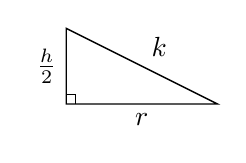
\begin{tikzpicture}[scale=0.8]
\draw[line width=0.5pt] (0,0) -- (2.4,0) -- (0,1.2) -- cycle; \draw[line width=0.4pt] (0,0.15)--(0.15,0.15)--(0.15,0);
\node[left] at (0,0.6) {$\frac{h}{2}$}; \node[below] at (1.2,0) {$r$}; \node[above right] at (1.2,0.6) {$k$};
\end{tikzpicture}}
% RVHS 2025 Promo Q1 solution diagram (conical tank with water)
\newcommand{\figRVHSsol}{\begin{tikzpicture}[scale=0.85]
\fill[blue!15] (-0.9,-1.5) -- (0,-3) -- (0.9,-1.5) arc[start angle=0,end angle=-180,x radius=0.9,y radius=0.15];
\draw[blue!50,fill=blue!8] (0,-1.5) ellipse (0.9 and 0.15);
\draw[c9] (0,0) ellipse (1.8 and 0.3); \draw[c9] (-1.8,0) -- (0,-3) -- (1.8,0);
\draw[c9aa] (0,0) -- (1.78,0); \node[above] at (0.9,0) {$3$};
\draw[c9aa] (-0.15,0) -- (-0.15,-3); \node[left] at (-0.15,-0.8) {$6$};
\draw[c9a] (0,-1.5) -- (0.88,-1.5); \node[above] at (0.45,-1.5) {$r$};
\draw[c9aa] (0.15,-1.5) -- (0.15,-3); \node[right] at (0.15,-2.2) {$h$};
\end{tikzpicture}}

\usepackage{multicol}
\usepackage{tikz-3dplot}\usepackage{colortbl}\usetikzlibrary{arrows.meta,positioning,shapes.geometric,calc}
\pgfplotsset{mini/.style={width=4.4cm,height=3.6cm,axis lines=middle,ticks=none,clip=false,xlabel=$x$,ylabel=$y$,label style={font=\small},unbounded coords=jump,every axis x label/.style={at={(ticklabel* cs:1)},anchor=west},every axis y label/.style={at={(ticklabel* cs:1)},anchor=south}},
noax/.style={width=4.8cm,height=4.4cm,axis lines=none,ticks=none,clip=false,axis equal image}}
\newcommand{\Om}{\node[anchor=north east,inner sep=1pt] at (axis cs:0,0){$O$};}
\newcommand{\ptt}[1]{\addplot[black,only marks,mark=*,mark size=1.2pt] coordinates{#1};}
\newcommand{\exg}[2]{\par\noindent\begin{minipage}[c]{0.54\textwidth}#1\end{minipage}\hspace{2mm}\begin{minipage}[c]{0.42\textwidth}\raggedright#2\end{minipage}\par\medskip}
\newcommand{\cell}[2]{\begin{minipage}[t]{0.32\textwidth}\centering#2\\[-1mm]{\small #1}\end{minipage}}
